%\title{LaTeX Portrait Poster Template}
%%%%%%%%%%%%%%%%%%%%%%%%%%%%%%%%%%%%%%%%%
% a0poster Portrait Poster
% LaTeX Template
% Version 1.0 (22/06/13)
%
% The a0poster class was created by:
% Gerlinde Kettl and Matthias Weiser (tex@kettl.de)
% 
% Adapter by Jens Buysse for Hogeschool Gent
% This template has been downloaded from:
% http://www.LaTeXTemplates.com
%
% License:
% CC BY-NC-SA 3.0 (http://creativecommons.org/licenses/by-nc-sa/3.0/)
%
%%%%%%%%%%%%%%%%%%%%%%%%%%%%%%%%%%%%%%%%%

%----------------------------------------------------------------------------------------
%	PACKAGES AND OTHER DOCUMENT CONFIGURATIONS
%----------------------------------------------------------------------------------------

\documentclass[a0,portrait]{a0poster}

\usepackage{multicol} % This is so we can have multiple columns of text side-by-side
\columnsep=100pt % This is the amount of white space between the columns in the poster
\columnseprule=3pt % This is the thickness of the black line between the columns in the poster

\usepackage[svgnames]{xcolor} % Specify colors by their 'svgnames', for a full list of all colors available see here: http://www.latextemplates.com/svgnames-colors

\usepackage{times} % Use the times font
%\usepackage{palatino} % Uncomment to use the Palatino font

\usepackage{graphicx} % Required for including images
\graphicspath{{figures/}} % Location of the graphics files
\usepackage{booktabs} % Top and bottom rules for table
\usepackage[font=small,labelfont=bf]{caption} % Required for specifying captions to tables and figures
\usepackage{amsfonts, amsmath, amsthm, amssymb} % For math fonts, symbols and environments
\usepackage{wrapfig} % Allows wrapping text around tables and figures
\usepackage[export]{adjustbox}

\begin{document}

%----------------------------------------------------------------------------------------
%	POSTER HEADER 
%----------------------------------------------------------------------------------------

% The header is divided into two boxes:
% The first is 75% wide and houses the title, subtitle, names, university/organization and contact information
% The second is 25% wide and houses a logo for your university/organization or a photo of you
% The widths of these boxes can be easily edited to accommodate your content as you see fit

\begin{minipage}[t]{0.75\linewidth}
\VeryHuge \color{HoGentAccent1} \textbf{ARM: van mobiele toestellen en IoT \\\\naar de desktop } \color{Black}\\ % Title
%\Huge\textit{Van mobiele toestellen en IoT naar de desktop}\\[2.4cm] % Subtitle
\\
\huge \textbf{Degryse Nathan, Mathieu Audenaert, Sharon Van Hove}\\[0.5cm] % Author(s)
\huge Hogeschool Gent, Valentin Vaerwyckweg 1, 9000 Gent\\[0.4cm] % University/organization
\Large \texttt{nathan.degryse@student.hogent.be} \\
\end{minipage}
%
\begin{minipage}[t]{0.25\linewidth}

\includegraphics[width=13cm,right]{figures/HOGENT_Logo_Pos_rgb.png} 

\end{minipage}

\vspace{1cm} % A bit of extra whitespace between the header and poster content

%----------------------------------------------------------------------------------------

\begin{multicols}{2} % This is how many columns your poster will be broken into, a portrait poster is generally split into 2 columns

%----------------------------------------------------------------------------------------
%	ABSTRACT
%----------------------------------------------------------------------------------------

\color{HoGentAccent1} % Navy color for the abstract

\begin{abstract}
Studenten en professionals hebben meestal geen oog voor technische details en specificaties wanneer ze een nieuwe laptop of desktop wensen aan te schaffen. Doorgaans hebben consumenten nood een toestel dat goed genoeg is om te voldoen aan hun specifieke eisen en gebruikssituaties. De nakende coëxistentie van ARM- en x86-processoren op het desktop-platform zal toekomstige kopers dwingen om na te denken over hun eigen unieke gebruiksscenario's en de behoefte aan softwareondersteuning voor de toepassingen die ze op een dagelijkse basis gebruiken. Die ondersteuning van software op meerdere processorarchitecturen zal de komende jaren steeds belangrijker worden voor zowel ontwikkelaars als consumenten.
\end{abstract}
%----------------------------------------------------------------------------------------
%	INTRODUCTION
%----------------------------------------------------------------------------------------

\color{HoGentAccent1} 
\section*{Introductie}
\color{black}
\color{black}
ARM processoren werden vroeger voornamelijk gebruikt in toestellen met een focus op mobiliteit en energiezuinigheid. Deze eisen zorgen ervoor dat ARM processors worden ontworpen met een focus op prestaties per watt. Dit concept is te verklaren als de hoeveelheid verwerkingscapaciteit die een processor/computer kan leveren per verbruikte watt aan energie. Het spreekt voor zich dat deze eigenschap de komende decennia een essentiële rol zal spelen bij het verlagen van het energieverbruik van individuele toestellen alsook het verlagen van de warmte uitstoot en het energieverbruik van datacenters. Tegenover de filosofie van de ARM processoren staat deze van het welbekende x86 platform die tot op de dag van vandaag dominant is in de markt van de desktop en laptop toestellen. Deze spitst zich toe op performantie en uitstekende software compatibiliteit.\\\\Deze verschillen zorgen ervoor dat er ook significante afwijkingen zijn op het gebied van het registergeheugen, de instructieset en software ondersteuning. De belangrijkste implicatie van dit gegeven is dat software die ontworpen en geschreven is voor het x86 platform niet compatibel is voor het ARM platform en vice versa. Dit houdt in dat softwareleveranciers meerdere versies van hun software moeten beschikbaar stellen om te voldoen aan de noden van hun klanten die gebruikmaken van verschillende hardware platformen. Vele softwaregiganten leveren uitstekende ondersteuning ongeacht het gekozen platform, maar toch is de compatibiliteit van de meeste software onvolmaakt of niet bestaande. Aangezien software specifiek moet geschreven worden voor het ARM platform, wegen de meeste softwareleveranciers de potentiële opbrengsten af tegenover de kosten die men moet spenderen aan het aanpassen van hun reeds bestaande software.

%----------------------------------------------------------------------------------------
%	GEOLOGY
%----------------------------------------------------------------------------------------

\color{Black} % DarkSlateGray color for the rest of the content
\color{HoGentAccent1} 
\section*{Experimenten}
\color{black}
Om te onderzoeken of desktops en laptops die gebruikmaken van een ARM processor een gebruikerservaring kunnen aanbieden die niet te onderscheiden valt van deze op een x86 toestel, heeft dit onderzoek drie ARM besturingssystemen onderworpen aan enkele testen. Scenario 1 is gericht op alledaags gebruik zoals browsen en kantoorsoftware.
In scenario 2 komen de geavanceerde ICT toepassingen aan bod die deel uitmaken van het dagelijkse softwarepakket van een student toegepaste informatica of een ICT professional. Tenslotte heeft een \textit{proof-of-concept} applicatie aangetoond dat het mogelijk is om een eenvoudige \textit{Swift} applicatie te schrijven die uitvoerbaar is op zowel iOS als macOS en dat met een minimum aan overtollige code of verlies aan performantie. Deze opstelling is mogelijk sinds 2020 dankzij de transitie van Intel x86 processoren naar de \textit{Apple Silicon} ARM architectuur.
\begin{center}\vspace{1cm}
	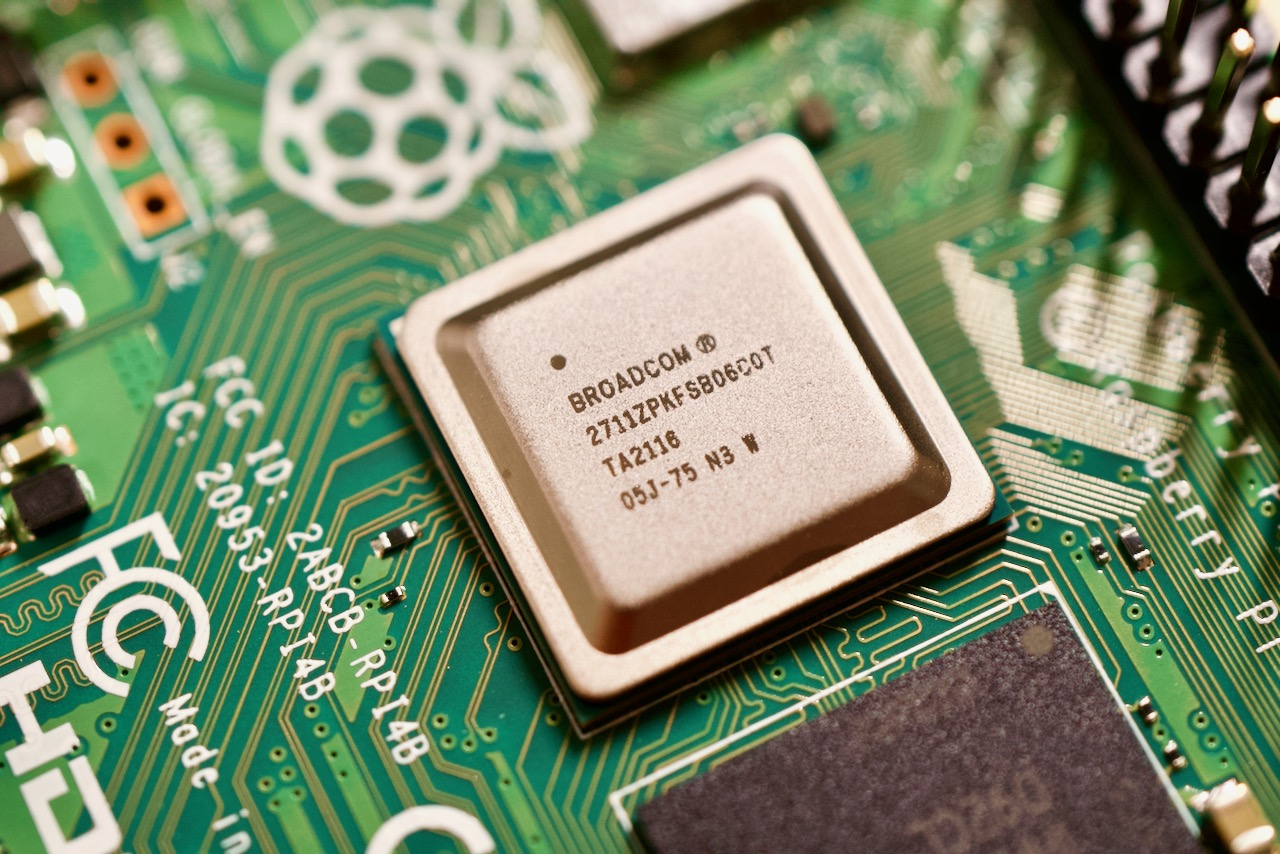
\includegraphics[width=1.0\linewidth]{pi4.jpeg}
	\captionof{figure}{\color{HoGentAccent5} Een overzicht van het moederbord van een Raspberry Pi 4B}
\end{center}\vspace{1cm}

\begin{center}\vspace{1cm}
\includegraphics[width=1.0\linewidth]{Apple_M1_Ultra_Family.png}
\captionof{figure}{\color{HoGentAccent5} Een overzicht van de eerste generatie aan \textit{Apple Silicon} processoren}
\end{center}\vspace{1cm}

%------------------------------------------------



\color{HoGentAccent1} 
\section*{Conclusies}
\color{black}
Dit onderzoek kan dienen als leidraad voor it-professionals of studenten die de overschakeling naar het ARM-platform wensen te maken. Dit platform is uitermate geschikt voor studenten en professionals die hun computer gebruiken voor alledaagse taken. Studenten en professionals met een informatica achtergrond kunnen de overstap maken naar een \textit{Apple Silicon} toestel indien men bereid is om grondig onderzoek te doen omtrent de software ondersteuning van de applicaties die nodig zijn voor hun alledaagse taken. Het gebrek aan software ondersteuning op het Windows on ARM platform zorgt ervoor dat deze toestellen op dit moment nog niet geschikt zijn voor consumenten met een focus op informatica. Alleen wanneer de software ondersteuning verbetert tot op het niveau van het Windows x86 platform, zullen deze doelgroepen in staat zijn om gebruik te maken van een Windows on ARM toestel.
%----------------------------------------------------------------------------------------
%	FORTHCOMING RESEARCH
%----------------------------------------------------------------------------------------
\color{HoGentAccent1} 
\section*{Toekomstig onderzoek}
\color{black}
Hoewel het ARM desktop platform nog relatief jong is, bevestigen technologie giganten zoals Apple en Microsoft hun overtuiging in dit platform door het jaarlijks uitbrengen van nieuwe hardware zoals de recent gelanceerde M2 \textit{Apple Silicon} chip en \textit{project Volterra}.  Het niveau van software ondersteuning is de afgelopen jaren exponentieel toegenomen en het is indrukwekkend hoe sommige professionals reeds gebruik kunnen maken van deze hardware voor hun alledaagse activiteiten. Om het huidige tempo van hardware- en software-innovatie op het ARM platform bij te houden, is het zinvol om deze studie te herhalen op jaarlijkse basis.


%----------------------------------------------------------------------------------------

\end{multicols}
\end{document}